% LaTeX source for ``การเรียนรู้ของเครื่องสำหรับเคมีควอนตัม (Machine Learning for Quantum Chemistry)''
% Copyright (c) 2022 รังสิมันต์ เกษแก้ว (Rangsiman Ketkaew).

% License: Creative Commons Attribution-NonCommercial-NoDerivatives 4.0 International (CC BY-NC-ND 4.0)
% https://creativecommons.org/licenses/by-nc-nd/4.0/

\chapter{วิธีเคอร์เนล}
\label{ch:kernel}

%--------------------------
\section{เคอร์เนลคืออะไร}
\label{sec:kernel}
\idxboth{เคอร์เนล}{Kernel}
%--------------------------

ในบทที่แล้วเราได้เรียนรู้เทคนิค Linear Regression (การถดถอยแบบเส้นตรง) กันไปแล้ว ซึ่งเป็นกรณีที่เราเจอปัญหาที่เกี่ยวข้องกับความสัมพันธ์%
ของตัวแปรสองตัว โดยเราสามารถทำการ Fit สมการเชิงเส้นของอินพุต ($x$) ให้เข้ากับชุดข้อมูล (Training Data) แล้วถ้าหากค่าเอาต์พุต 
($y$) ที่เราต้องการทำนายนั้นสามารถถูกทำนายหรืออธิบายได้ดีกว่าด้วยสมการไม่เชิงเส้น (Nonlinear Function) ของตัวแปร $x$ นั้น 
เราสามารถใช้สิ่งที่เรียกว่าเคอร์เนล (Kernel) ซึ่งเราจะมาเรียนรู้กันในบทนี้ 

\begin{figure}[htbp]
    \centering
    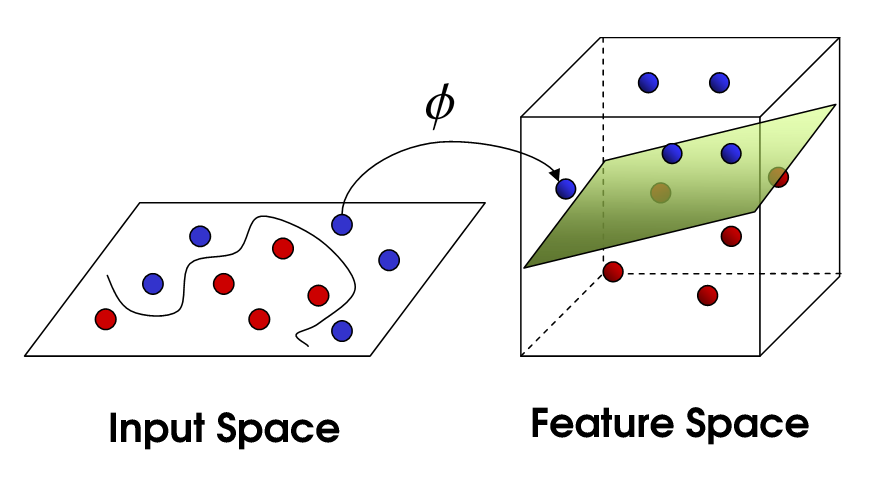
\includegraphics[width=0.8\linewidth]{fig/2d_to_3d_spaces.png}
    \caption{การทำ Mapping จากปริภูมิ 2 มิติไปเป็นปริภูมิ 3 มิติซึ่ง Observation ของเราสามารถถูกแยกได้โดยฟังก์ชันเชิงเส้น}
    \label{fig:2d_to_3d}
\end{figure}

ถ้าสมมติว่าผู้เขียนเริ่มต้นด้วยการยกสมการทางคณิตศาสตร์มาอธิบายว่าเคอร์เนลคืออะไร ผู้อ่านหลายท่านก็อาจจะสับสนได้ ดังนั้นผู้จึงขอยกเริ่มต้นด้วย%
การอธิบายง่าย ๆ แบบนี้ว่าถ้าสมมติเรามีชุดข้อมูลที่อยู่ในปริภูมิ 2 มิติ (2-dimensional Space) หรือที่เรียกว่า Input Space ดังที่แสดงในภาพที่ 
\ref{fig:2d_to_3d} เราจะพบว่าเราไม่สามารถหาฟังก์ชันเชิงเส้นที่สามารถแยกข้อมูลจุดสีแดงออกจากสุดสีน้ำเงินได้ แต่ถ้าหากเราแปลงข้อมูล%
จากปริภูมิ 2 มิติให้ไปอยู่ในปริภูมิ 3 มิติซึ่งเราจะเรียกปริภูมินี้ว่า Feature Space ตามรูปทางด้านขวา เราพบว่าข้อมูลของเราหลังจากที่ถูกแปลงนั้น%
จะสามารถถูกแยกออกจากกันได้ด้วยฟังก์ชันเชิงเส้น (ในที่นี้คือระนาบที่แบ่งข้อมูลทั้งสองคลาสออกจากกัน) ซึ่งกระบวนการนี้เรียกว่า Mapping 
หลังจากนั้นให้เราทำ Mapping อีกครั้งหนึ่งโดยแปลงย้อนกลับไปสู่ปริภูมิ 2 มิติ ซึ่งผลลัพธ์ที่ได้จะเป็นฟังก์ชันแบบไม่เชิงเส้นที่อยู่ในมิติที่ต่ำลงนั่นเอง 
\idxen{Mapping}

สรุปสั้น ๆ คือวิธีเคอร์เนลเป็นการประยุกต์ใช้ฟังก์ชันเชิงเส้นกับปัญหาที่เป็นแบบไม่เชิงเส้นโดยการแปลงข้อมูลให้อยู่ในปริภูมิที่มีมิติที่สูงขึ้น (อาจจะ 3 
มิติหรือสูงกว่านี้ก็ได้) โดยที่เราไม่จำเป็นที่จะต้องเข้าใจปริภูมิมิติสูงเหล่านั้น

%--------------------------
\section{คณิตศาสตร์ของเคอร์เนล}
\label{sec:math_kernel}
%--------------------------

ก่อนที่เราจะลงลึกไปที่ตัวทฤษฎีของเคอร์เนลนั้น เราควรจะต้องมาทำความเข้าใจสิ่งที่เป็นพื้นฐานกันก่อนนั่นก็คือ Feature Map ซึ่งเป็นสิ่งที่ทำการ%
เชื่อมโยง Attribute ให้เข้ากับ Feature ซึ่งเราเรียกกระบวนการนี้ว่า Mapping ตามที่ได้อธิบายไปก่อนหน้านี้

เริ่มต้นด้วยการพิจารณาการ Fit ฟังก์ชันแบบ Cubic Function โดยสมการดังนี้

\begin{equation}\label{eq:cubic_func}
    y = \theta_{3}x^{3} + \theta_{2}x^{2} + \theta_{1}x^{1} + \theta_{0}
\end{equation}

\noindent จะเห็นได้ว่าเราสามารถที่จะมอง Cubic Function ด้านบนเป็นสมการเชิงเส้นง่าย ๆ ซึ่งสมการ \ref{eq:cubic_func} นั้นจะขึ้น%
อยู่กับ Feature Variables ($x$) ที่เรากำหนดไว้นั่นเอง คราวนี้เราลองมากำหนดฟังก์ชันใหม่โดยอ้างอิงสมการเดิม ซึ่งเราจะมีการกำหนดเซต%
ของตัวแปร $x$ ตัวใหม่ขึ้นมานั่นคือ

\begin{align}\label{eq:cubic_func_2}
    y &= \theta_{3}x^{3} + \theta_{2}x^{2} + \theta_{1}x^{1} + \theta_{0} \nonumber \\ 
      &= \theta^{\top}\phi(x)
\end{align}

\noindent โดยที่ $\phi$ คือเวกเตอร์ของตัวแปรอินพุต ดังนี้

\begin{equation}
\phi = 
\begin{bmatrix}
    1 \\
    x \\
    x^{2} \\
    x^{3} 
\end{bmatrix}
\end{equation}

\noindent และ $\theta^{\top}$ เป็นเวกเตอร์ของพารามิเตอร์ $\theta_{i}$ ดังนี้

\begin{equation}
\theta^{\top} =
\begin{bmatrix}
    \theta_{o} & \theta_{1} & \theta_{2} & \theta_{3}
\end{bmatrix}
\end{equation}

\noindent ซึ่งทั้งสองเวกเตอร์นี้ก็คูณกันแบบ Dot Product ตามสมการที่ \ref{eq:cubic_func_2}
 
คำถามที่ตามมาก็คือเราจะแยกความแตกต่างระหว่างสมการ \ref{eq:cubic_func} กับ \ref{eq:cubic_func_2} ได้อย่างไร คำตอบก็คือเรา%
สามารถทำได้โดยการกำหนดให้ตัวแปรอินพุต $x$ ของเรานั้นเป็น Attribute เมื่อเราทำการ Map หรือเชื่อมโยงตัวแปร $x$ ของเราไปยังปริมาณ%
ตัวใหม่ที่เป็น $\phi(x)$ เราจะเรียกปริมาณตัวนี้ว่า Feature และฟังก์ชันที่เราใช้ในการ Mapping นั้นเราเรียกว่า Feature Map ($\phi$) 
ซึ่งเป็นตัวที่ทำการเชื่อมโยงความสัมพันธ์ของ Attribute ไปยัง Feature ตามที่ได้เกริ่นไว้ก่อนหน้านี้

ดังนั้นโจทย์ของเราในการทำ Regression ก็คือการหาอัลกอริทึม Gradient Descent ที่จะนำมาใช้ในการ Fitting โมเดลของเรา (อันที่จริงแล้ว
$\theta^{\top}\phi(x)$ ก็คือโมเดลของเรานั่นเอง) โดยหนึ่งในอัลกอริทึมที่สามารถนำมาใช้ในการ Fitting ได้อย่างมีประสิทธิภาพก็คือ 
Stochastic Gradient Descent ซึ่งมีสมการดังต่อไปนี้

\begin{equation}\label{eq:sto_grad_des}
    \theta := \theta + \alpha (y^{i} - \theta^{\top}\phi(x^{i}))\phi(x^{i})
\end{equation}

\noindent โดยที่ $\alpha$ คือขนาดของการก้าวเดิน (Step Size) หรืออัตราเร็วของการเรียนรู้ (Learning Rate) ซึ่งเป็นพารามิเตอร์ที่จะ%
ปรับความเร็วในการปรับความเหมาะสม (Optimize) เกรเดียนต์ (สำหรับรายละเอียดเพิ่มเติมเกี่ยวกับการพิสูจน์สมการที่ \ref{eq:sto_grad_des} 
ผู้อ่านสามารถอ่านได้จากหนังสือปัญญาประดิษฐ์) อย่างไรก็ตาม ปัญหาอย่างหนึ่งของ Stochastic Gradient Descent นั้นก็คือไม่สามารถที่จะ%
หาผลเฉลยได้ง่าย จึงทำให้การฝึกสอนโมเดลนั้นมีความสิ้นเปลืองในการคำนวณเป็นอย่างมาก (Computationally Expensive) โดยเฉพาะอย่าง%
ยิ่งเมื่อ Feature ของเรา ($\phi(x)$) นั้นมีจำนวนมิติที่เยอะมาก ๆ (ผู้อ่านสามารถศึกษารายละเอียดของ Stochastic Gradient Descent 
ได้ในหัวข้อที่ \ref{ssec:stochastic_grad})

สำหรับนิยามของเคอร์เนล ($K$) นั้นจริง ๆ แล้วมีหลายนิยามมาก ขึ้นอยู่กับว่าต้องการจะให้นิยามในบริบททางคณิตศาสตร์หรือสถิติ โดยส่วนตัวของ%
เขียนนั้นคิดว่าเคอร์เนลเป็นวิธีทางสถิติที่เกี่ยวข้องกับการหาความเชื่อมโยงระหว่างตัวแปรสองตัว ซึ่งความเชื่อมโยงในที่นี้ก็คือความคล้ายคลึงกัน 
(Similarity) ผู้อ่านบางท่านอาจจะเคยได้ยินหรือเคยใช้วิธี เช่น Jaccard Similarity หรือ Cosine Similarity มาก่อนบ้าง 

คราวนี้เรามาดูนิยามทางคณิตศาสตร์ของเคอร์เนลกันครับ เริ่มต้นกำหนดเคอร์เนลให้อยู่ในรูปของ Feature Map ($\phi$) ซึ่งเป็นฟังก์ชันที่ทำการ 
Mapping ปริภูมิของตัวแปรอินพุต $x$ ที่ได้อธิบายไว้ก่อนหน้านี้ ($\chi \times \chi \rightarrow \mathbb{R}$) ดังนี้

\begin{equation}\label{eq:kernel}
    K(x,z) = \langle\phi(x),\phi(z)\rangle
\end{equation}

\noindent ซึ่งเราสามารถคำนวณ $\langle\phi(x),\phi(z)\rangle$ ได้โดยการใช้สมการต่อไปนี้

\begin{align}
    \langle\phi(x),\phi(z)\rangle =& 1 + \sum_{i=1}^d x_i z_i + 
    \sum_{i,j\in\{1,\ldots,d\}} x_i x_j z_i z_j \nonumber \\
    &+ \sum_{i,j,k \in \{1,\ldots,d\}} x_i x_j x_k z_i z_j z_k \\
    =& 1 + \sum_{i=1}^d x_i z_i + \left(\sum_{i=1}^d x_i z_i \right)^2 + \left( \sum_{i=1}^d x_i z_i \right)^3 \\
    =& 1 + \langle x,z \rangle + \langle x,z \rangle^2 + \langle x,z \rangle^3\label{eq:feat_map_inner_product}
\end{align}

\noindent อธิบายง่าย ๆ ก็คือเราจะคำนวณพจน์แรก $\langle x,z \rangle$ ของสมการ \ref{eq:feat_map_inner_product} ก่อน 
หลังจากนั้นจึงคำนวณพจน์อื่น ๆ ที่เหลือ (กำหนดให้ $i,j$ เป็นสมาชิกของเซต $\{1, \dots, n\}$)

%--------------------------
\section{ฟังก์ชันเคอร์เนลและคุณสมบัติของเคอร์เนล}
\label{sec:func_kernel}
\idxboth{เคอร์เนล!ฟังก์ชันเคอร์เนล}{Kernel!Function Kernel}
\idxen{Kernel!Kernel Properties}
%--------------------------

ในหัวข้อนี้เราจะมาดูรายละเอียดของเคอร์เนลกันว่า $K(x,z)$ มีคุณสมบัติอะไรที่น่าสนใจบ้าง สำหรับสัญลักษณ์ที่เราจะกำหนดขึ้นมาเพื่ออธิบาย%
เคอร์เนลนั้นจะเป็น $K(\cdot,\cdot)$ หรือเรียกง่าย ๆ ว่าเป็นฟังก์ชันเคอร์เนล (Kernel Function) ก็ได้ ผู้เขียนขอยกตัวอย่างของฟังก์ชัน%
เคอร์เนลแบบเรียบง่ายให้ดูกันก่อน ดังนี้

\begin{equation}
    K(x,z) = (x^{\top} z)^{2}
\end{equation}

\noindent ซึ่งเราสามารถจัดรูปสมการใหม่ได้เป็น

\begin{align}
    K(x,z) &= \left( \sum_{i=1}^d x_i z_i \right) \left( \sum_{j=1}^d x_j z_j \right)\\
    &= \sum_{i=1}^d \sum_{j=1}^d x_i x_j z_i z_j\\
    &= \sum_{i,j=1}^d (x_i x_j)(z_i z_j)
\end{align}

\noindent ซึ่งจะเห็นได้ชัดเลยว่าจริง ๆ แล้วนั้น $K(x,z) = \langle\phi(x),\phi(z)\rangle$ เป็นฟังก์ชันเคอร์เนลที่สอดคล้องกับ Feature 
Mapping ($\phi$) โดยที่มีสมการเป็น (กรณีที่ $d = 3$)

\begin{equation}\label{eq:feature_map_ex1}
    \phi(x) = \begin{bmatrix}
    x_1 x_1\\
    x_1 x_2\\
    x_1 x_3\\
    x_2 x_1\\
    x_2 x_2\\
    x_2 x_3\\
    x_3 x_1\\
    x_3 x_2\\
    x_3 x_3\\
    \end{bmatrix}
\end{equation}

เราลองมาดูตัวอย่างที่สองของ $K(\cdot,\cdot)$ ซึ่งถูกกำหนดด้วยฟังก์ชันเชิงเส้นดังต่อไปนี้

\begin{align}
    K(x,z) &= (x^{\top} z + c)^2\\
    &= \sum_{i,j=1}^d (x_i x_j)(z_i z_j) + \sum_{i=1}^d \left(\sqrt{2c}x_i\right) \left(\sqrt{2c}z_i\right) 
    + c^2
\end{align}

\noindent โดยที่ฟังก์ชันเคอร์เนลด้านบนนี้ก็จะคล้าย ๆ กับก่อนหน้านี้แต่จะมีความแตกต่างตรงที่มีการเพิ่มพารามิเตอร์ $c$ เข้ามา ซึ่งเป็นสิ่งที่%
กำหนดการถ่วงน้ำหนัก (Weighting) ระหว่าง $x_{i}$ และ $x_{i}x_{j}$ โดยที่เรามองได้ง่าย ๆ ก็คือเคอร์เนล $K(x,z) = (x^{\top} 
z + c)^2$ นั้นจะมีความสอดคล้องกับ Feature Mapping ไปยังปริภูมิของ $\binom{d+k}{k}$ โดยที่ Feature Mapping ของกรณีนี้นั้นมี%
สมการดังต่อไปนี้ (กรณีที่ $d = 3$))

\begin{equation}\label{eq:feature_map_ex2}
    \phi(x) = \begin{bmatrix}
        x_1 x_1\\
        x_1 x_2\\
        x_1 x_3\\
        x_2 x_1\\
        x_2 x_2\\
        x_2 x_3\\
        x_3 x_1\\
        x_3 x_2\\
        x_3 x_3\\
        \sqrt{2c}x_1\\
        \sqrt{2c}x_2\\
        \sqrt{2c}x_3\\
        c
    \end{bmatrix}
\end{equation}

\begin{figure}[htbp]
    \centering
    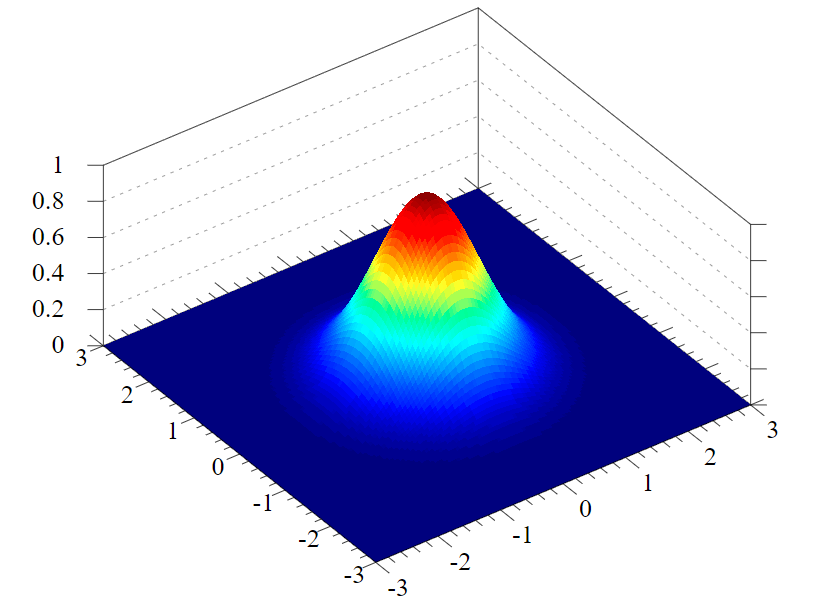
\includegraphics[width=0.9\linewidth]{fig/gaussian-3d.png}
    \caption{ตัวอย่างพื้นผิวการกระจายตัวเกาส์เซียน (Gaussian Distribution) ในปริภูมิ 3 มิติ}
    \label{fig:gaussian_3d}
\end{figure}

คราวนี้เราลองมามองเคอร์เนลให้เป็นเมตริกหรือตัววัดความคล้ายคลึงกันระหว่าง Feature Mapping (Similarity Metrics) เราเริ่มต้นด้วย%
สมมติฐานที่ว่าถ้ากรณีที่ $\phi(x)$ กับ $\phi(z)$ บนปริภูมินั้นมีความใกล้กันมาก ๆ เราอาจจะคาดการณ์ได้ว่า $K(x,z) = \phi(x)^{\top} 
\phi(z$ จะมีขนาดที่ใหญ่มากเพราะว่ามีการซ้อนทับกันเยอะ (เรานิยามให้การซ้อนทับกันหรือ Overlap นั้นเป็นความคล้ายคลึงกัน) แต่ในกรณีที่%
ตรงข้ามกัน ถ้าหาก $\phi(x)$ กับ $\phi(z)$ อยู่ห่างกันมากก็จะทำให้การ Overlap นั้นมีน้อย จึงทำขนาดของเคอร์เนล $K(x,z) = 
\phi(x)^{\top} \phi(z)$ มีขนาดที่เล็กลงตามไปด้วย ซึ่งการที่เราสามารถนิยามเคอร์เนลให้เป็นมาตรวัดความคล้ายคลึงกันระหว่าง $x$ และ 
$z$ นั้นมีประโยชน์อย่างมาก เพราะเราสามารถนำไปแก้ปัญหาหลาย ๆ อย่างได้ แต่ว่าฟังก์ชันที่เราเลือกมาใช้ในการอธิบายความแตกต่างของทั้งสอง%
ตัวแปรนั้นจะต้องมีความสมเหตุสมผล โดยฟังก์ชันที่ได้รับความนิยมในการนำมาใช้เป็นฟังก์ชันเคอร์เนลนั้นก็คือฟังก์ชันเกาส์เซียน (Gaussian 
Function) หรือเรียกอีกอย่างว่า Radial BasisFunction (RBF) ตามภาพที่ \ref{fig:gaussian_3d} ซึ่งมีสมการดังต่อไปนี้ 

\begin{equation}\label{eq:rbf_kernel}
    K(x,z) = \exp\left(-\frac{\lVert x - z \rVert^2}{2\sigma^2}\right)   
\end{equation}

\noindent โดยที่ $\sigma$ คือไฮเปอร์พารามิเตอร์ (Hyperparameter) ที่กำหนดความเรียบเนียน (Smoothness) ของขอบเขตการตัดสินใจ 
(Decision Boundary) และ $\lVert x - z \rVert^2$ คือระยะห่างยูคลิเดียนยกกำลังสอง (Squared Euclidean Distance) ระหว่าง 
Feature Vector $x$ และ $z$ ซึ่งสามารถหาค่าได้โดยใช้สมการดังต่อไปนี้

\begin{align}
    d(x_{i}, x_{k}) &= 
    \sqrt{(x^{(1)}_{i} - x^{(1)}_{k})^{2} + (x^{(2)}_{i} - x^{(2)}_{k})^{2} + \cdots + 
    (x^{(N)}_{i} - x^{(N)}_{k})^{2}} \\
    &= \sqrt{\sum^{N}_{n=1} (x^{(n)}_{i} - x^{(n)}_{k})^{2}}
\end{align}

ฟังก์ชันในสมการ \ref{eq:rbf_kernel} นั้นเมื่อถูกนำมาใช้เป็นเคอร์เนลแล้วเราจะเรียกเคอร์เนลนี้ว่าเคอร์เนลเกาส์เซียน (Gaussian Kernel)
ซึ่งเป็นฟังก์ชันที่เหมาะสมมาก ๆ เพราะว่ามีความสมมาตร มีความต่อเนื่องตลอดช่วงของปริภูมิ และมีค่าเข้าใกล้ 1 เมื่อ $x$ และ $z$ นั้นอยู่ใกล้กัน 
แต่จะมีค่าเข้าใกล้ 0 เมื่อ $x$ และ $z$ อยู่ห่างกัน

เรามาดูการเขียนโค้ดสำหรับการ Mapping ด้วยวิธีเคอร์เนลกันครับ เริ่มต้นด้วยโค้ดที่กำหนดชุดข้อมูลตัวอย่างซึ่งเป็นแบบไม่เป็นเชิงเส้น ดังนี้

\begin{lstlisting}[style=MyPython]
import numpy as np
import matplotlib.pyplot as plt

# Kernel
x = np.array([1,1,2,3,3,6,6,6,9,9,10,11,12,13,16,18])
y = np.array([18,13,9,6,15,11,6,3,5,2,10,5,6,1,3,1])
label = np.array([1,1,1,1,0,0,0,1,0,1,0,0,0,1,0,1])

# Plot
fig = plt.figure()
plt.scatter(x, y, c=label, s=60)
plt.show()
\end{lstlisting}

\noindent เขียนฟังก์ชันสำหรับการ Mapping ดังนี้

\begin{lstlisting}[style=MyPython]
def mapping(x, y):    
	x = np.c_[(x, y)]				
    if len(x) >	2:        
    	x_1 = x[:,0]**2        
        x_2 = np.sqrt(2)*x[:,0]*x[:,1]        
        x_3 = x[:,1]**2								
    else:            
    	x_1 = x[0]**2        
        x_2 = np.sqrt(2)*x[0]*x[1]        
        x_3 = x[1]**2			    
    trans_x = np.array([x_1, x_2, x_3])				
    return trans_x	
\end{lstlisting}

\noindent แล้วทำการ Mapping, แสดงผลลัพธ์ และพล็อตข้อมูลหลังจาก Mapping

\begin{lstlisting}[style=MyPython]
# Mapping
x_1  = mapping(x, y)
x_1.shape
# Output
(3, 15)

# Plot
fig = plt.figure()
ax = fig.add_subplot(111, projection='3d')
ax.scatter(x_1[0], x_1[1], x_1[2], c=label, s=60)
ax.view_init(30, 185)
ax.set_xlabel('X Label')
ax.set_ylabel('Y Label')
ax.set_zlabel('Z Label')
plt.show()
\end{lstlisting}

โดยสรุปก็คือเคอร์เนลเป็นเทคนิคอย่างหนึ่งที่ช่วยให้เราสามารถทรานฟอร์มหรือแปลงข้อมูล (Transform) จากปริภูมิมิติต่ำ (Low-dimensional 
Space) ไปยังปริภูมิมิติสูง (High-dimensional Space) ซึ่งฟังก์ชันที่เหมาะสมที่สุดที่เราสามารถเลือกมาใช้เป็นฟังก์ชันเคอร์เนลได้นั้นไม่มีใครรู้%
ว่ามีหน้าตาเป็นอย่างไร ดังนั้นการที่เราจะทำ Mapping โดยเลือกใช้ทุกฟังก์ชันนั้นจึงแทบจะเป็นไปไม่ได้เลยเพราะว่ามีขีดจำกัดด้านการคำนวณ

%--------------------------
\subsection{การถดถอยแบบเชิงเส้น}
\label{ssec:lin_reg}
\idxen{Kernel!Linear Regression}
%--------------------------

กรณีแบบแรกของการถดถอย (Regression) ก็คือการถดถอยแบบเชิงเส้น (Linear Regression) ซึ่งเราได้ศึกษากันไปแล้วในหัวข้อที่ 
\ref{sec:lin_res} ของบทที่ \ref{ch:sup_ml} ซึ่งเราใช้สมการดังต่อไปนี้ในการแก้ปัญหาการปรับค่าลงให้ต่ำที่สุด (Minimization)

\begin{equation}
    \min_{w} \lVert X_{w} - y \rVert_{2}^{2}
\end{equation}

\begin{figure}[htbp]
    \centering
    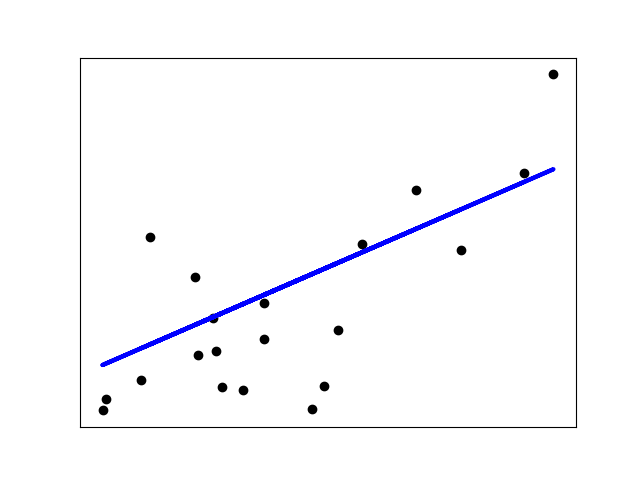
\includegraphics[width=0.8\linewidth]{fig/plot_linear_regression.png}
    \caption{เส้นตรงที่ถูก Fit (สมดุล) ให้ผ่านจุดในชุดข้อมูล แกน $x$ คืออินพุตและแกน $y$ คือเอาต์พุต (เครดิตภาพ: 
    https://scikit-learn.org)}
    \label{fig:lin_res}
\end{figure}

รูปที่ \ref{fig:lin_res} แสดงเส้นตรงที่เกิดจากการทำ Minimization ของสมการถดถอยแบบเชิงเส้น เส้นตรงสีน้ำเงินเส้นนี้ถูกปรับระยะห่าง%
เฉลี่ยระหว่างจุดทุกจุดในชุดข้อมูลโดยที่มีความสมดุลมากที่สุด โดยสังเกตด้วยตาเปล่าได้คร่าว ๆ ว่าแนวโน้มของจุดนั้นจะมีแนวโน้มที่เป็นแบบเอียง%
และชันขึ้นจากทางด้านซ้ายไปยังด้านขวา ดังนั้นเส้นตรงที่ได้จากการ Fit นั้นจึงมีแนวโน้มไปในทางเดียวกันซึ่งมีความชันเป็นบวกนั่นเอง

%--------------------------
\subsection{การถดถอยแบบริดจ์}
\label{ssec:ridge_reg}
\idxth{การถดถอย!การถดถอยแบบริดจ์}
\idxen{Kernel!Ridge Regression}
%--------------------------

สำหรับวิธีการถดถอยแบบริดจ์ (Ridge Regression) นั้นอาจจะมองได้ว่าเป็นการยกระดับ (Upgrade) หรือปรับปรุง Linear Regression 
ในกรณีที่เป็นแบบสามัญ (Ordinary) ให้มีประสิทธิภาพมากขึ้น นั่นก็เพราะว่ากรณีที่เราจะต้องทำการ Fit ข้อมูลที่มีจำนวนหลายตัวแปรและมีการ%
กระจายในแบบที่ไม่สามารถอธิบายได้ด้วยสมการเส้นตรงนั้น เรามีเทคนิคก็คือการใส่พจน์พิเศษเข้าไป ซึ่งวิธีนี้เรียกว่าเป็นการลงโทษ (Penalize) 
ซึ่งเป็นหนึ่งในรูปแบบของการทำ Regularization โดยมีรูปสมการทั่วไปดังต่อไปนี้

\begin{equation}
    \min_{w} \lVert X_{w} - y \rVert_{2}^{2} + \alpha \lVert w \rVert_{2}^{2}
\end{equation}

\noindent โดยพระเอกของเราใน Ridge Regression นั้นก็คือพจน์สุดท้ายซึ่งมีศัพท์ทางเทคนิคที่เรียกว่า $L2$ Regularization โดยมี%
พารามิเตอร์ที่สำคัญนั่นก็คือ $\alpha$ ซึ่งเป็นตัวปรับจำนวนการหด (Schrinkage) ของฟังก์ชัน ซึ่งคูณอยู่กับค่าขนาดของน้ำหนัก (Weight) 
ยกกำลังสอง ซึ่งการยกกำลังนี้เป็นที่มาของการเรียกว่า $L2$ นั่นเอง สำหรับวิธีการปรับค่า $\alpha$ และผลกระทบที่เกิดขึ้นนั้นสามารถดูได้ตามรูปที่ 
\ref{fig:ridge_res}

\begin{figure}[htbp]
    \centering
    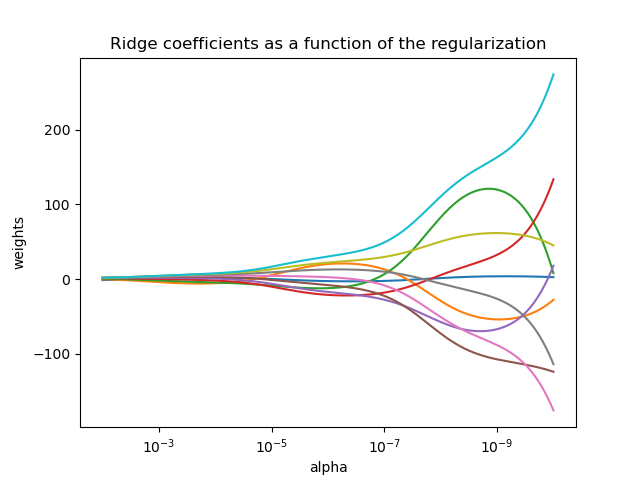
\includegraphics[width=0.9\linewidth]{fig/plot_ridge_regression.png}
    \caption{สัมประสิทธิ์ของริดจ์ที่เป็นฟังก์ชันกับ Regularization (เครดิตภาพ: https://scikit-learn.org)}
    \label{fig:ridge_res}
\end{figure}

\noindent โดยเราจะพบว่ายิ่ง $\alpha$ มีค่ามากเท่าไหร่ จำนวนของการขดของฟังก์ชันหรือเส้นโค้งก็จะมีจำนวนมากตามไปด้วย (เช่นเส้นสีส้ม) 
ดังนั้นค่าสัมประสิทธิ์ที่มีความซับซ้อนขึ้นนั้นก็จะยิ่งส่งผลดีต่อการนำไปอธิบายชุดข้อมูลที่มีความไม่เป็นเส้นตรงสูง

อธิบายเสริม: กรณีที่การทำ Regularization ไม่ได้ใช้การยกกำลังสองของค่าขนาดของน้ำหนักแต่ใช้เพียงแค่ยกกำลังหนึ่งนั้น เราจะเรียกเทคนิคนี้ว่า
LASSO ซึ่งย่อมาจาก Least Absolute Shrinkage and Selection Operator หรือเรียกสั้น ๆ ว่า $L1$ โดยมีสมการดังนี้

\begin{equation}
    \min_{w} \lVert X_{w} - y \rVert_{2}^{2} + \alpha \lVert w \rVert_{1}
\end{equation}

%--------------------------
\section{การถดถอยแบบริดจ์ด้วยเคอร์เนล}
\label{sec:kernel_ridge}
\idxth{การถดถอย!การถดถอยแบบริดจ์ด้วยเคอร์เนล}
\idxen{Kernel!Kernel Ridge Regression}
%--------------------------

การถดถอยแบบริดจ์ด้วยเคอร์เนล (Kernel Ridge Regression หรือ KRR) เป็นการต่อยอดจาก Ridge Regression หรืออธิบายง่าย ๆ ว่า 
KRR ก็คือ RR ในเวอร์ชั่นที่เป็น Nonlinear Problem ซึ่งมีการผสม Kernel Trick เข้าไปด้วย (Kernel + Ridge Regression) 
โดยรูปแบบของโมเดลที่ถูกสอนให้เรียนรู้โดย KRR นั้นก็ยังมีรูปแบบอื่น ๆ แยกย่อยไปอีกหลายเทคนิค เช่น เทคนิค Support Vector Regression 
(SVR) โดยความแตกต่างระหว่าง KRR กับ SVM ก็คือการใช้ Loss Function ที่ต่างกัน โดย KRR จะใช้ค่า Loss Error ยกกำลังสอง ในขณะที่ 
SVR จะใช้ $\epsilon$-incentive Loss

นอกจากนี้ยังมีเทคนิคอื่น ๆ อีกที่อาศัยหลักการของ Kernel Trick โดยหนึ่งในนั้นก็คือ Gaussian Process Regression ซึ่งถูกนำมาใช้ในการ%
พัฒนาเทคนิค Gaussian Approximation Potential (GAP) ซึ่งเป็นเทคนิคที่มีการใช้อย่างแพร่หลายโดยเฉพาะการศึกษาการทำนายพลังงาน%
รวมของโมเลกุล\autocite{bartok2010,bartok2015}

%--------------------------
\section{การถดถอยแบบกระบวนการเกาส์เซียน}
\label{sec:gaussian_process}
\idxth{การถดถอย!การถดถอยแบบกระบวนการเกาส์เซียน}
\idxen{Kernel!Gaussian Process Regression}
%--------------------------

การถดถอยแบบกระบวนการเกาส์เซียน (Gaussian Process Regression หรือ GPR) เป็นเทคนิคที่มีความคล้ายกับ KRR นั่นก็คือทำการเรียนรู้
ฟังก์ชันคำตอบ (Target Function) ของโดยการใช้ Kernel Trick เหมือนกัน แต่ว่าจะมีความแตกต่างกันก็คือในกรณีของ KRR นั้นจะทำการ%
เรียนรู้ฟังก์ชันเชิงเส้นในในปริภูมิที่ถูกสร้างขึ้นมาใหม่ด้วยเคอร์เนลที่เรากำหนดเข้าไปซึ่งจะสอดคล้องหรือเชื่อมโยงกับฟังก์ชันแบบไม่เป็นเชิงเส้นในปริภูมิเดิม 
ซึ่งฟังก์ชันเชิงเส้นในปริภูมิของเคอร์เนลนั้นก็จะขึ้นอยู่กับ Loss Function (ในกรณีทั่วไปคือ Mean Square Error) กับ Ridge Regularization 
ในกรณีของ GPR นั้นจะเป็นการใช้เคอร์เนลในการกำหนดความแปรปรวนร่วม (Covariance) ของการแจกแจงก่อน (Prior Distribution) 
ซึ่ง Covariance นี้เป็นพารามิเตอร์ที่สามารถบ่งบอกถึงแนวโน้มของข้อมูลว่ามีการเปลี่ยนแปลงไปในทิศทางเดียวกันมากน้อยแค่ไหน กล่าวง่าย ๆ 
ก็คือ GPR จะเป็นการพยายามที่จะมาเล่นกับ Covariance มากกว่าจะเป็นการทำนายฟังก์ชันคำตอบและใช้ชุดข้อมูลที่ใช้ในการฝึกสอนโมเดลมาทำ%
การกำหนดฟังก์ชันที่ควรจะเป็น (Likelihood Function) นอกจากนี้แล้ว GPR ยังใช้หลักการของ Bayes Theorem ซึ่งจะมีการกำหนดการ%
แจกแจงภายหลัง (Posterior Distribution) โดยใช้ Gaussian Function เพื่อนำค่าเฉลี่ยมาใช้ในการทำนายคำตอบอีกด้วย

\begin{figure}[htbp]
    \centering
    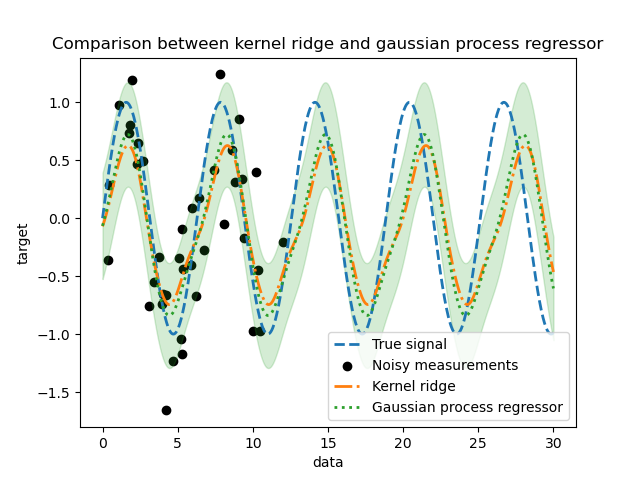
\includegraphics[width=0.9\linewidth]{fig/plot_gpr_kernel.png}
    \caption{เปรียบเทียบการเรียนรู้ Target ระหว่างเทคนิค KRR และ GPR (เครดิตภาพ: https://scikit-learn.org)}
    \label{fig:krr_gpr}
\end{figure}

ภาพที่ \ref{fig:krr_gpr} แสดงการเปรียบเทียบความแม่นยำในการทำนายค่า Target ระหว่าง KRR (เส้นสีส้ม) และ GPR (เส้นประสีเขียว) 
และมีค่าอ้างอิง (เส้นประสีฟ้า) เป็นตัวชี้วัดความแม่นยำ โดยสรุปได้ว่า GPR มีความแม่นยำและความถูกต้องในการทำนายเทียบเท่าพอ ๆ กับ KRR 
ตลอดช่วงของจำนวนข้อมูล เมื่อเราทำการเพิ่มขนาดของชุดข้อมูลจะพบว่าโมเดลทั้งสองอันจะให้ค่าที่ยังสอดคล้องกันแต่จะ Deviate ออกห่างจาก%
ค่าอ้างอิงมากขึ้นเรื่อย ๆ 

รายละเอียดของ Gaussian Process นั้นมีเยอะมาก ถ้าหากผู้อ่านสนใจศึกษาเพิ่มเติมเกี่ยวกับทฤษฎีเชิงลึกและคณิตศาสตร์ที่ใช้ในการอธิบายวิธีนี้%
ผู้เขียนแนะนำหนังสือ \textit{Gaussian Processes for Machine Learning} ของ Carl Edward Rasmussen และ 
Christopher K. I. Williams ซึ่งสามารถอ่านและดาวน์โหลดได้ฟรีที่ \url{http://gaussianprocess.org/gpml}
